\documentclass[12pt]{article}
\usepackage{graphicx} %package to manage images
\graphicspath{ {./figures/} }
\usepackage{caption}
\usepackage[font=scriptsize]{subcaption}
\captionsetup[figure]{labelsep=none}
\captionsetup[table]{labelsep=none}
\usepackage{bbm}
\usepackage{amsmath}
\usepackage{import}
\usepackage{array}
\usepackage{booktabs}
\usepackage{afterpage}
\usepackage{floatrow}
\usepackage{pdflscape}
\usepackage{soul}
\usepackage{float}
\usepackage{adjustbox}
\usepackage{longtable}
\usepackage{caption}
\usepackage{setspace}
\usepackage{afterpage}
\usepackage[margin=1in]{geometry}
\usepackage[round]{natbib}
\usepackage{hyperref}
\usepackage{titlesec}

\title{EGC Stata Test 070625 S278}
\author{Sidh Pandit}
\date{August 2025}

\begin{document}

\maketitle


\subsection{part c}

\begin{table}[H]
    \centering
    \scriptsize % shrink text
    \setlength{\tabcolsep}{2pt}
    \renewcommand{\arraystretch}{2}
    \resizebox{\textwidth}{!}{{
\def\sym#1{\ifmmode^{#1}\else\(^{#1}\)\fi}
\begin{tabular}{l*{3}{cccccc}}
\hline\hline
            &\multicolumn{6}{c}{hhinc\_topcoded}                                           &\multicolumn{6}{c}{log\_hhinc\_topcoded}                                       &\multicolumn{6}{c}{log\_hhinc\_topcoded}                                       \\
            &        Mean&          SD&   1st pctl.&      Median&  99th pctl.&         Max&        Mean&          SD&   1st pctl.&      Median&  99th pctl.&         Max&        Mean&          SD&   1st pctl.&      Median&  99th pctl.&         Max\\
\hline
\hline
\(N\)       &        4160&            &            &            &            &            &        3916&            &            &            &            &            &        3584&            &            &            &            &            \\
\hline\hline
\multicolumn{19}{l}{\footnotesize 24-month income is estimated by 24*household income in last 30 days.}\\
\end{tabular}
}
}
    \caption{: Endline raw data summary statistics}
\end{table}


The average per-capita income for households in the sample is \$1.02 a day, which is well below the international extreme poverty threshold. 

There is large variation and inequality in household income and per-capita income - in both cases the mean is almost twice the median, suggesting a right skewed distribution.

Indeed, there are extreme outliers, with maximum values exceeding the 99th percentile at large orders of magnitude. Similar patterns hold for both formal and informal borrowing.


\begin{figure}[H]
    \centering
    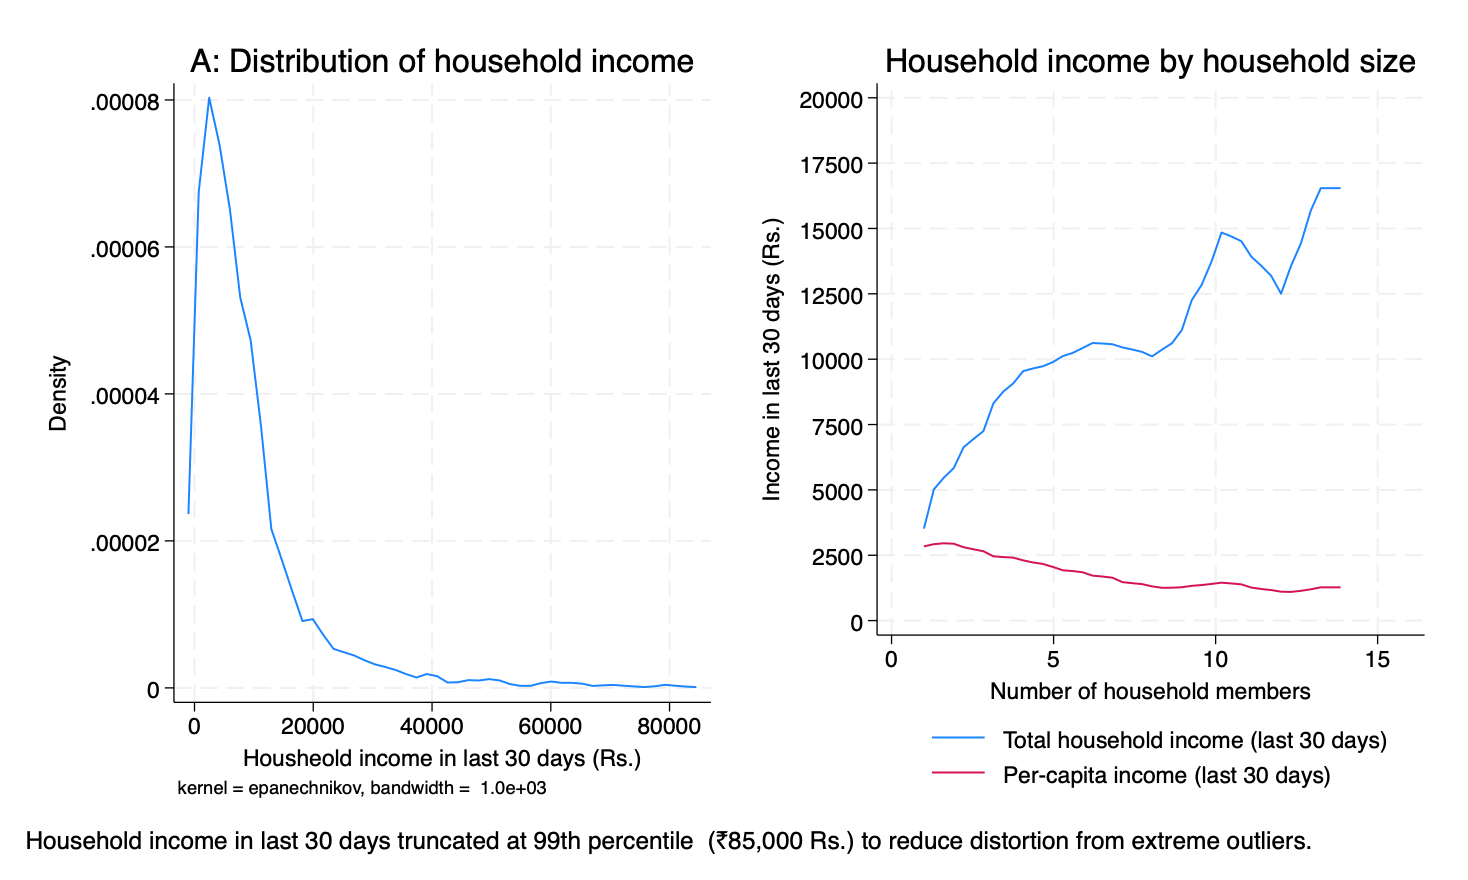
\includegraphics[width=\textwidth]{figures/figure01_hhinc.png}
    \caption{: Distribution and composition of household income in last 30 days}
\end{figure}

Panel A visually confirms the skewed distribution even excluding the top percentile.

Panel B illustrates that while household income was positively correlated with household size, per-capita income was negatively correlated with household size.


\begin{figure}[H]
    \centering
    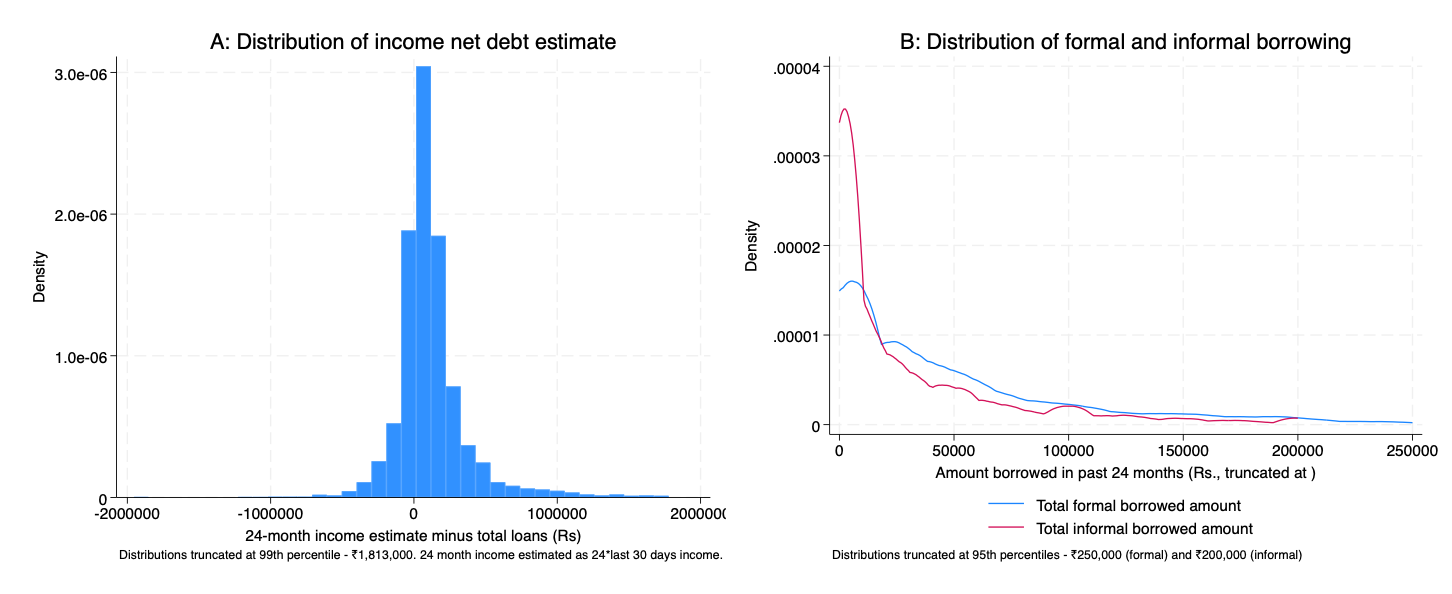
\includegraphics[width=\textwidth]{figures/figure02_loandistribution.png}
    \caption{: Distribution of total borrowing (loans) in last 24 months}
\end{figure}

Here we can see that informal borrowing is much more common


\subsection{part f}

top code so that upper end of the distribution is censored

large outliers skew stuff
might be measurement error or self reported bias or recall bias

check for extreme debt to income ratios 


\subsection{part j}

strengths of the dummy
- per-capita


weaknesses of the dummy
- ask about expenses to build local poverty line, perhaps nutrition based



\subsection{part k}

drop all baseline only - not even part of experiment

endline only not significantly different by treated or control

\section{part 2: analysis}

\subsection{part a}

testable hypothesis about impacts of the program on an outcome or subgroup

Early expansion of banks increased total formal borrowing among sc/st households less than other households

\subsection{part b}

Why did you choose these particular variables to test?

What are the results of the test, and what can they tell us about the validity of the
experiment?


- social groups: stark inequality in institutional access/ awareness
- gender of hoh: migration patterns differ by village
- age of hoh: joint household status may differ by village
- education: none, primary, secondary, higher (collapse years of education into categorical variables)
- literacy: attainment vs attendance
- no. household members
- no. hh members above 18 years
- no. hh members below 18 years



\section{References used}

\end{document}
